\documentclass{article}
\usepackage[T2A]{fontenc}
\usepackage[utf8]{inputenc}
\usepackage{graphicx}

\title{Документация по игре Тетрис}
\author{rosscome}

\begin{document}

\maketitle

\section*{Логика игры}

\subsection*{Введение}
Тетрис "--- это классическая аркадная игра, разработанная Алексеем Пажитновым в 1984 году. Игра стала одной из самых известных и популярных в истории видеоигр благодаря своей простой, но в то же время захватывающей игровой механике.

\subsection*{Игровой процесс}
Игрок управляет падающими тетромино (фигурами, состоящими из четырех квадратных блоков), которые могут вращаться и перемещаться горизонтально в пределах игрового поля. Цель игры "--- заполнять горизонтальные линии блоками без пропусков. Когда заполняется целая линия, она исчезает, освобождая место для новых блоков. Игра заканчивается, когда столбцы блоков достигают верхней части поля.

\subsection*{Основные элементы игры}
\begin{itemize}
    \item \textbf{Тетромино}: Фигуры, состоящие из четырех квадратных блоков. Всего существует семь различных типов тетромино.
    \item \textbf{Игровое поле}: Прямоугольная сетка, в которой падают и размещаются тетромино.
    \item \textbf{Управление}: Игрок управляет тетромино с помощью клавиш управления (например, стрелок) для перемещения вправо, влево, поворота и ускорения падения.
    \item \textbf{Очки и уровни}: Игра ведет подсчет очков в зависимости от заполненных линий. Чем больше линий одновременно заполняется, тем больше очков получает игрок. Уровень увеличивается с набором определенного количества очков, что повышает скорость падения тетромино.
    \item \textbf{Выход из игры}: Игрок может завершить игру по желанию, либо начать заново после окончания текущей игры.
\end{itemize}

\subsection*{Цель игры}
Цель игры Тетрис заключается в том, чтобы получить как можно больше очков, заполняя горизонтальные линии и избегая достижения верхней границы игрового поля.

\subsection*{Заключение}
Тетрис остается популярной игрой благодаря своей простой и захватывающей игровой механике, которая требует от игрока стратегического мышления и быстрых реакций. Игра доступна на множестве платформ и является одной из самых узнаваемых видеоигр в мире.

\section*{Конечный автомат игры}

\begin{figure}[h]
    \centering
    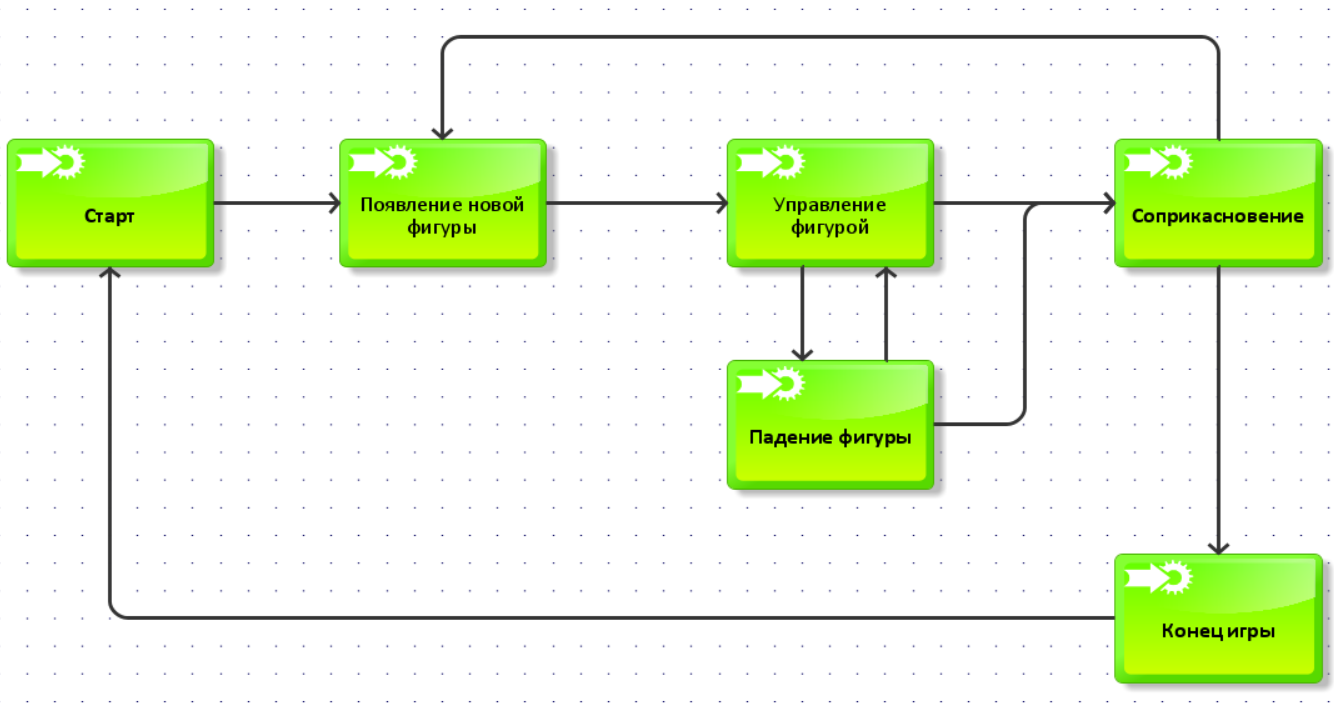
\includegraphics[width=1\textwidth]{../misc/images/fsm.png}
    \caption{КА игры Тетрис}
    \label{fig:example}
\end{figure}


Данный КА состоит из следующих состояний:

Старт — состояние, в котором игра ждет, пока игрок нажмет кнопку готовности к игре.

Спавн — состояние, в которое переходит игра при создании очередного блока и выбора следующего блока для спавна.

Перемещение — основное игровое состояние с обработкой ввода от пользователя — поворот блоков/перемещение блоков по горизонтали.

Сдвиг — состояние, в которое переходит игра после истечения таймера. В нем текущий блок перемещается вниз на один уровень.

Соединение — состояние, в которое преходит игра после «соприкосновения» текущего блока с уже упавшими или с землей. Если образуются заполненные линии, то она уничтожается и остальные блоки смещаются вниз. Если блок остановился в самом верхнем ряду, то игра переходит в состояние «игра окончена».

Игра окончена — игра окончена.

\end{document}
